\documentclass[xcolor=dvipsnames]{beamer}
\usepackage{amsmath}
\usetheme{Warsaw}
\usecolortheme[named=Brown]{structure}
\beamertemplatenavigationsymbolsempty


\begin{document}
 \title{GetMyBio.me}
 \subtitle{...but I don't give a shit}
 \author{Sai, Aditya, Justin, Jana}
 
 
  \begin{frame}
    \titlepage
    \begin{center}
     \includegraphics[scale=0.7]{HPILogo.png}
    \end{center}
  \end{frame}
  
  \begin{frame}
    \frametitle{The microbiome defines YOU}
    	\begin{columns}
	    	\begin{column}{.6\textwidth}
	    	\includegraphics[scale=0.5]{symbio.png}
	    	\end{column}
	    	\begin{column}{.4\textwidth}
	    	\begin{itemize}
	    	\item Changes with life(style)
	    	\item Risk indicator for diseases
	    	\item Personalised (probiotic) diet
	    	\end{itemize}
	    	\end{column}
    	\end{columns}
    	 	
  \end{frame}
  
  \begin{frame}
      \frametitle{Microbiome insights for individuals}
      \begin{columns}
      		\begin{column}{.7\textwidth}
      		\includegraphics[scale=0.5]{innovation.png}
            \end{column}
            \begin{column}{.3\textwidth}
            	\textbf{Advantages:}
            	\begin{itemize}
            		\item no culture system
            		\item not influenced by salts
            		\item rapid
            	\end{itemize}
            \end{column}
      \end{columns}
    \end{frame}

	\begin{frame}
      \frametitle{Our prototype with visible "bacteria"}
      \begin{columns}
      \begin{column}{.5\textwidth}
      Achievements:
            \begin{itemize}
            	\item Image analysis 
            	\item Retrieve proportions of colored bacteria
            	\item Android app
            \end{itemize}
            \vspace{\baselineskip}
            Outlook:
                  \begin{itemize}
                  	\item Generate ultra-sound with more Hz 
                  	\item Staining protocol for baceria
                  	\item Connection to database
                  \end{itemize}
      \end{column}
      \begin{column}{.5\textwidth}
      	 \begin{center}
      	  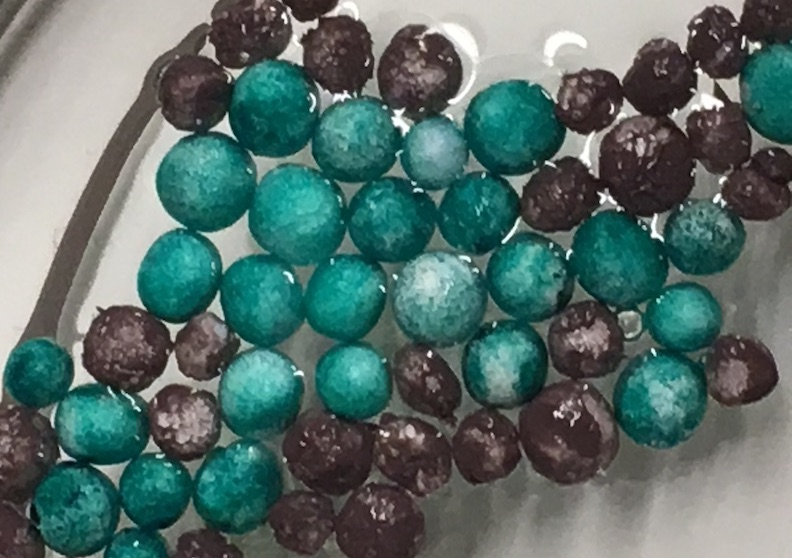
\includegraphics[scale=0.1]{bacteria-mag.jpg}\newline
      	  \vspace{0.5cm}\newline
      	  \includegraphics[scale=0.3]{hist.png}
      	 \end{center}
      \end{column}
      \end{columns}
    \vspace{\baselineskip} 
     
    \end{frame}
    
    \begin{frame}
    \begin{center}
    e\mbox{-}Health at home
    \vspace{2cm}
    
    Save your stool, just drool.\newline
    \includegraphics[scale=0.5]{end.png}
    \end{center}
    \end{frame}
    
    \begin{frame}
    References:
    \vspace{\baselineskip}
    \newline
    Zourob M, Hawkes JJ, Coakley TW ,Treves Brown BJ, Fielden PR, McDonnell MB and Goddard NJ (2005) Optical Leaky Waveguide Sensor for Detection of Bacteria with Ultrasound Attractor Force. \textit{Anal. Chem.} \textbf{77}, pp 6163\mbox{-}6168.\\
    \vspace{1cm}
    http://www.homd.org
    
    \end{frame}

\end{document}